\subsection{Total Kinetic Energy in a Collection of Particles}
\begin{definition}[Total Kinetic Energy]
	\label{def:total-kinetic-energy}
	In a discrete system of N particles with {\bf mass} $m_i$ and position vector $\underline{r_i}\left(t  \right) $, the {\bf total kinetic energy} of a collection of particles is defined as
	\begin{equation}
		\label{eq:total-kinetic-energy}
		K_{tot} = \sum\limits_{i=1}^{N}\frac{1}{2}m_{i} \mid \underline{\dot{r}}_{i}\mid ^{2}
	\end{equation}
\end{definition}

\clearpage
Consider the following diagram (R is the center of mass \ref{eq:com}):
\begin{mycenter}
	\tikzset{every picture/.style={line width=0.75pt}} %set default line width to 0.75pt        

	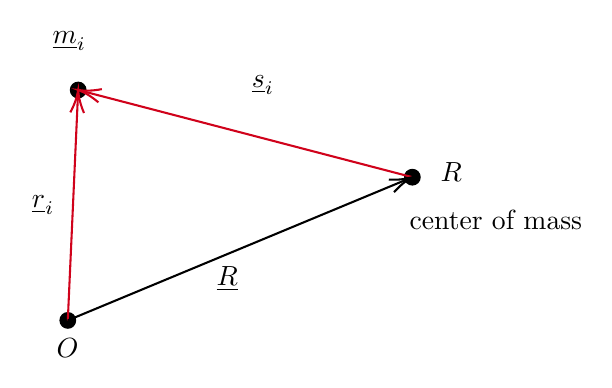
\begin{tikzpicture}[x=0.75pt,y=0.75pt,yscale=-1,xscale=1]
		%uncomment if require: \path (0,300); %set diagram left start at 0, and has height of 300

		%Shape: Circle [id:dp3521186394752994] 
		\draw  [fill={rgb, 255:red, 0; green, 0; blue, 0 }  ,fill opacity=1 ] (129.3,194.53) .. controls (129.3,192.58) and (130.88,191) .. (132.83,191) .. controls (134.78,191) and (136.37,192.58) .. (136.37,194.53) .. controls (136.37,196.48) and (134.78,198.07) .. (132.83,198.07) .. controls (130.88,198.07) and (129.3,196.48) .. (129.3,194.53) -- cycle ;
		%Shape: Circle [id:dp11213586931309727] 
		\draw  [fill={rgb, 255:red, 0; green, 0; blue, 0 }  ,fill opacity=1 ] (134.3,83.53) .. controls (134.3,81.58) and (135.88,80) .. (137.83,80) .. controls (139.78,80) and (141.37,81.58) .. (141.37,83.53) .. controls (141.37,85.48) and (139.78,87.07) .. (137.83,87.07) .. controls (135.88,87.07) and (134.3,85.48) .. (134.3,83.53) -- cycle ;
		%Shape: Circle [id:dp673844600958276] 
		\draw  [fill={rgb, 255:red, 0; green, 0; blue, 0 }  ,fill opacity=1 ] (295.3,125.53) .. controls (295.3,123.58) and (296.88,122) .. (298.83,122) .. controls (300.78,122) and (302.37,123.58) .. (302.37,125.53) .. controls (302.37,127.48) and (300.78,129.07) .. (298.83,129.07) .. controls (296.88,129.07) and (295.3,127.48) .. (295.3,125.53) -- cycle ;
		%Straight Lines [id:da6095891694092731] 
		\draw [color={rgb, 255:red, 208; green, 2; blue, 27 }  ,draw opacity=1 ]   (132.83,194.53) -- (137.74,85.53) ;
		\draw [shift={(137.83,83.53)}, rotate = 92.58] [color={rgb, 255:red, 208; green, 2; blue, 27 }  ,draw opacity=1 ][line width=0.75]    (10.93,-3.29) .. controls (6.95,-1.4) and (3.31,-0.3) .. (0,0) .. controls (3.31,0.3) and (6.95,1.4) .. (10.93,3.29)   ;
		%Straight Lines [id:da032325149412671395] 
		\draw [color={rgb, 255:red, 208; green, 2; blue, 27 }  ,draw opacity=1 ]   (298.83,125.53) -- (139.77,84.04) ;
		\draw [shift={(137.83,83.53)}, rotate = 14.62] [color={rgb, 255:red, 208; green, 2; blue, 27 }  ,draw opacity=1 ][line width=0.75]    (10.93,-3.29) .. controls (6.95,-1.4) and (3.31,-0.3) .. (0,0) .. controls (3.31,0.3) and (6.95,1.4) .. (10.93,3.29)   ;
		%Straight Lines [id:da15576096830380182] 
		\draw    (132.83,194.53) -- (296.99,126.3) ;
		\draw [shift={(298.83,125.53)}, rotate = 157.43] [color={rgb, 255:red, 0; green, 0; blue, 0 }  ][line width=0.75]    (10.93,-3.29) .. controls (6.95,-1.4) and (3.31,-0.3) .. (0,0) .. controls (3.31,0.3) and (6.95,1.4) .. (10.93,3.29)   ;

		% Text Node
		\draw (126,202) node [anchor=north west][inner sep=0.75pt]   [align=left] {$\displaystyle O$};
		% Text Node
		\draw (311,117) node [anchor=north west][inner sep=0.75pt]   [align=left] {$\displaystyle R$};
		% Text Node
		\draw (114,133) node [anchor=north west][inner sep=0.75pt]   [align=left] {$\displaystyle \underline{r}_{i}$};
		% Text Node
		\draw (220,75) node [anchor=north west][inner sep=0.75pt]   [align=left] {$\displaystyle \underline{s}_{i}$};
		% Text Node
		\draw (296,140) node [anchor=north west][inner sep=0.75pt]   [align=left] {center of mass};
		% Text Node
		\draw (124,54) node [anchor=north west][inner sep=0.75pt]   [align=left] {$\displaystyle \underline{m}_{i}$};
		% Text Node
		\draw (203,167) node [anchor=north west][inner sep=0.75pt]   [align=left] {$\displaystyle \underline{R}$};


	\end{tikzpicture}

\end{mycenter}

Set $\underline{s}_{i} = \underline{r}_{i} - \underline{R}$, then

\begin{align*}
	K_{tot} = \frac{1}{2}\sum\limits_{i=1}^{N}m_{i}\mid \underline{\dot{r_{i}}} \mid^{2} & \Rightarrow K_{tot} = \frac{1}{2} \sum\limits_{i=1}^{N}m_{i}\mid \underline{\dot{R}} +\underline{\dot{s_{i}}} \mid^2                                                                                  \\ \\
                                                                                       & \Rightarrow K_{tot} = \frac{1}{2}\sum\limits_{i=1}^{N}\Big[m_{i}\mid \underline{\dot{R}} \mid^{2} + m_{i}2\underline{\dot{R}} \cdot \underline{s_{i}} +m_{i}\mid \underline{\dot{s}_{i}} \mid\Big] \label{eq: si-zero}\tag{1}
\end{align*}

\begin{note}
	From the definition of the {\bf center of mass} \eqref{eq:com}, we have

	$$\begin{aligned} M\underline{R} = \sum\limits_{i=1}^{N}m_{i}\underline{r_{i}} & = \sum\limits_{i=1}^{N} m_{i}(\underline{R} + \underline{s_{i}}) \\ \\
                                                                             & = M\underline{R} + \sum\limits_{i=1}^{N}m_{i}\underline{s_{i}}\end{aligned}$$
	and therefore, we get
	$$\sum\limits_{i=1}^{N}m_{i}\underline{s_{i}} = 0$$
\end{note}
and therefore, \eqref{eq: si-zero} becomes
$$K_{tot} = \frac{1}{2}M\mid\underline{\dot{R}} \mid^{2} + \frac{1}{2}m_{i}\mid \underline{\dot{s}_{i}}\mid^{2}$$
where $M = \sum\limits_{i=1}^{N}$

\begin{definition}[Total Kinetic Energy v2]
	In a discrete system of N particles with {\bf mass} $m_i$ and position vector $\underline{r_i}\left(t  \right) $, the {\bf total kinetic energy} of a collection of particles is defined as
	\begin{equation}
		\label{eq:total-kinetic-energy-2}
    K_{tot} = \frac{1}{2}M\mid\underline{\dot{R}} \mid^{2} + \frac{1}{2}\sum_{i=1}^{N}m_{i}\mid \underline{\dot{s}_{i}}\mid^{2}
	\end{equation}

\end{definition}

\clearpage
